\documentclass{mp}
\graphicspath{{07_rozklady/}}
\subtitle{Przykładowe rozkłady prawdopodobieństwa}
\begin{document}
\frame{\titlepage}

\begin{frame}{Rozkład dwupunktowy}
\only<1-2>
{
\begin{center}
\begin{tikzpicture}
\node[dice] (root) {?}
	child { node [diagram,below left=of root.center] {$X=-2$} edge from parent node[left] {$\leq 2$}}
	child { node [diagram,below right=of root.center] {$X=3$} edge from parent node[right] {$> 2$}};
\end{tikzpicture}
\end{center}
\[ P(X=-2)=\alert<1>{?} \qquad P(X=3)=\alert<1>{?} \]
}
\only<2->
{
\begin{block}{}
\begin{align*}
P(X=a)=p & \qquad P(X=b)=1-p \\
EX=\alert<2>{?} & \qquad DX=\alert<2>{?}
\end{align*}
\end{block}
\begin{block}<3->{Rozkład zero-jedynkowy}
\begin{align*}
P(X=1)=p & \qquad P(X=0)=1-p \\
EX=\alert<3>{?} & \qquad DX=\alert<3>{?}
\end{align*}
\end{block}
}
\end{frame}


\begin{frame}{Rozkład geometryczny}
\tabcolsep=0cm
\begin{tabular}{cccccccccc}
\includegraphics[width=.1\textwidth]{head.jpg} &
\includegraphics[width=.1\textwidth]{head.jpg} &
\includegraphics[width=.1\textwidth]{head.jpg} &
\includegraphics[width=.1\textwidth]{head.jpg} &
\includegraphics[width=.1\textwidth]{head.jpg} &
\includegraphics[width=.1\textwidth]{head.jpg} &
\includegraphics[width=.1\textwidth]{head.jpg} &
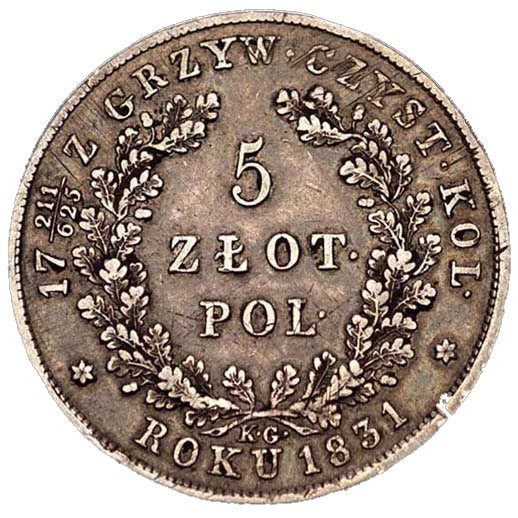
\includegraphics[width=.1\textwidth]{tail.jpg} &
\end{tabular}
\begin{gather*}
P(K=k)=(1-p)^{k-1}p \qquad k\in\{1,2,\ldots\} \\
EK=\frac{1}{p} \qquad DK=\frac{\sqrt{1-p}}{p}
\end{gather*}
\end{frame}
\begin{frame}{Rozkład dwumianowy (Bernouliego)}
\tabcolsep=0cm
\begin{tabular}{cccccccccc}
\includegraphics[width=.1\textwidth]{head.jpg} &
\includegraphics[width=.1\textwidth]{head.jpg} &
\includegraphics[width=.1\textwidth]{head.jpg} &
\includegraphics[width=.1\textwidth]{head.jpg} &
\includegraphics[width=.1\textwidth]{head.jpg} &
\includegraphics[width=.1\textwidth]{head.jpg} &
\includegraphics[width=.1\textwidth]{head.jpg} &
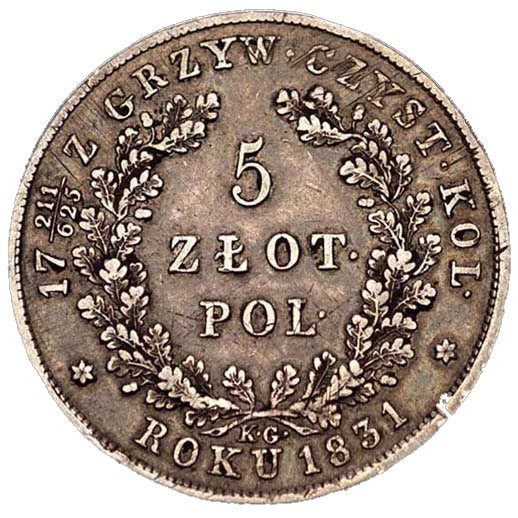
\includegraphics[width=.1\textwidth]{tail.jpg} &
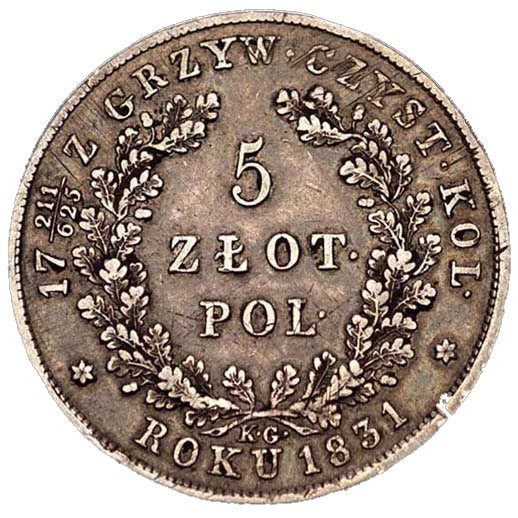
\includegraphics[width=.1\textwidth]{tail.jpg} &
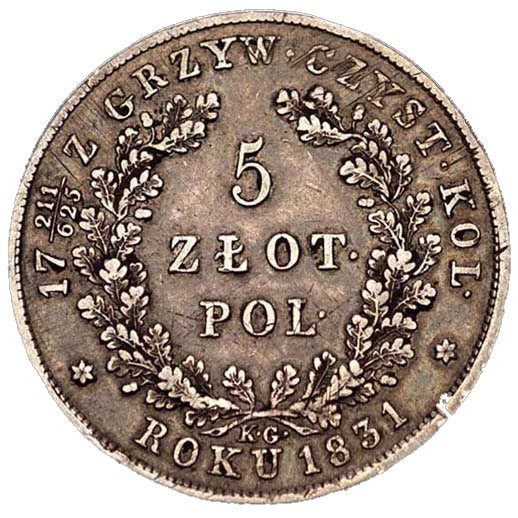
\includegraphics[width=.1\textwidth]{tail.jpg} \\
$X_1$ & $X_2$ & $X_3$ & $X_4$ & $X_5$ & $X_6$ & $X_7$ & $X_8$ & $X_9$ & $X_{10}$ \\
\end{tabular}
\begin{gather*}
P(X_i=1)=p \qquad P(X_i=0)=1-p \\
\only<2->{K=X_1+X_2+\ldots+X_n \\}
\only<3->{
	P(K=k)=\only<-5>{\alert<4->{?}}\only<6->{{n \choose k}}\only<5->{p^k(1-p)^{n-k}} \qquad k\in\{\only<3>{\alert{?}}\only<4->{0,1,\ldots,n}\}\\
}
\only<7->
{
	EK=\alert{?}\qquad DK=\alert{?}
}
\end{gather*}
\vfill
{\tiny Zdjecie monety z \url{http://commons.wikimedia.org/wiki/File:Powstanie_listopadowe_5_z\%C5\%82otych_1831.JPG} by \emph{Niki K} CC BY-SA 3.0}
\end{frame}
\begin{frame}{Rozkład Poissona}
\begin{tikzpicture}
\foreach \x in {0,...,49}
	\foreach \y in {0,...,4}
	\node at ($\x*(.02\textwidth,0)+\y*(0,.02\textwidth)$) {\ifnum \y<3 \includegraphics[width=.019\textwidth]{head.jpg}\else 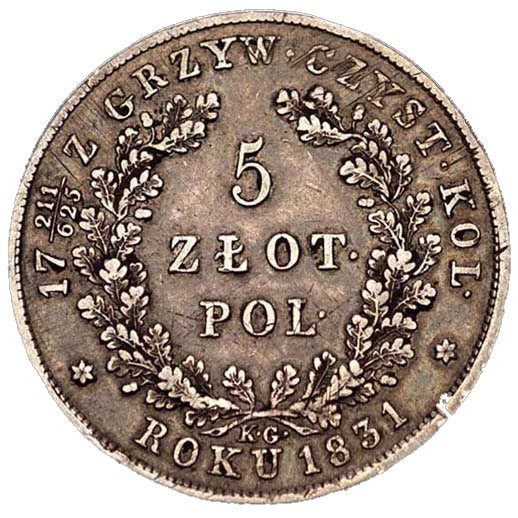
\includegraphics[width=.019\textwidth]{tail.jpg}\fi};
\end{tikzpicture}
\begin{gather*}
P(X=k)=e^{-\lambda}\frac{\lambda^k}{k!} \qquad k\in\{0,1,\ldots\}\quad \lambda\in\mathbb{R}_{+} \\
\only<2->{EX=\lambda\qquad DX=\sqrt{\lambda}}
\end{gather*}
\begin{block}<3->{Przybliżenie rozkładu Bernouliego rozkładem Poissona}
\[ \left( n\geq 50 \land p\leq 0{,}1 \land np\leq 10 \right) \to B(n,p)\approx Pois(np) \]
\end{block}
\end{frame}
\begin{frame}{Tablice rozkładu Poissona}
\small
\tabcolsep=0.1cm
\input{poisson.tex}
\end{frame}
\end{document}
